\section{Personal-PCFG, an individual oriented password cracker}
\label{personalpcfg}
We have presented abundant findings regarding user personal information and their passwords, as well as a metric to quantify their correlation. Naturally we wonder how these findings are useful. An obvious answer is that given there is significant correlation between user password and personal information, much potential can be seen to crack passwords faster. To this end, we create Personal-PCFG, which relies on the idea of PCFG approach created by M. Weir \cite{weir2009password}. However, unlike original PCFG method, Personal-PCFG is an individual-oriented password cracker, which generates personalized guesses towards each user. Note that we do not claim to be the first trying to leverage personal information to crack passwords. OMEN+ \cite{castelluccia2013privacy}, which improves Markov Models \cite{narayanan2005fast} to crack passwords, has done simple experiment to prove usefulness of personal information. However, we do not consider this work well done because 1) The experiment is done on only 3,140 users with personal information both insufficient and unreliable. 2) Personal information is not treated ``personally" -- they are simply divided into 3-grams and the probabilities of these 3-grams are raised up a little in the attack dictionary. 3) Dividing personal information into 3-grams internally break the continuation of personal information and causes many coincidences. 

We believe the effect of OMEN+ \cite{castelluccia2013privacy} is roughly equivalent to adding common names, locations, etc to training data. It tries to use personal information of individual user to generate guesses for all users, which is by its nature improper. 

\subsection{Attack Scenarios}
Personal-PCFG can be used in both offline and online attacks. We assume that the attacker knows certain amount of personal information about the targets. The attackers can be an evil neighbor, a curious friend, a jealous husband, a blackmailer, or even a company that buys personal information from other companies. We argue that under these conditions, target personal information is rather easy to obtain -- The attackers might either know the victim personally or can easily get personal information by searching online, especially on social networks sites (SNS). 

In traditional offline password attacks, attackers usually steal hashed passwords from victim systems, and try to find out the unhashed values of these passwords. As hash process cannot be simply reversed, the most usual solution is by brute force, namely guessing and verifying passwords. Every guess is verified by hashing the guess (salt is also likely to be added) and comparing the result to the hashed values. high-probability password guesses can usually match many hashed values and thus are expected to be tried first. In offline attacks, Personal-PCFG is much faster in guessing out the correct password than conventional methods by generating high-probability personalized passwords.

As for online attack, the attacker does not even have a hashed database. Instead the attacker tries to directly log in the real systems by guessing the passwords. It is considered more difficult than offline attacks because service systems usually have restrictions on log in attempts for a given period of time. If the attempt quota has been reached without inputting the correct password, the target account may be locked either for some time or permanently unless certain actions are taken (For example, call the service provider). As a matter of fact, online attacks need to be very fast -- within at most tens of guesses the password should be cracked out. Personal-PCFG is able to crack 1 out of 20 passwords within only 5 guesses. 

\subsection{A revisit of PCFG}
Personal-PCFG is based on the idea of PCFG method. Before we introduce Personal-PCFG. We revisit the basic principle of PCFG method. PCFG method pre-processes passwords by their structures. From the pre-process, base structures such as $"L_5D_3S_1"$ are generated for each of the passwords. Starting from high-probability structures, PCFG method substitutes the ``D" and ``S" segments using segments of same length learned from the training set. These substitute segments are ranked by probability of occurring in training set. Therefore higher probability segments will be tried first. As a result, one base structure may have many substitutions, for example, $"L_5D_3S_1"$ can have $"L_5123!"$ and $"L_5691!"$, etc as its substitutions. These new representations are called pre-terminal structures. No ``L" segment is currently substituted because the space of alpha strings is too large to learn from the training set. These pre-terminals are ranked from high probability to low probability. And finally ``L" segments are substituted using a dictionary. Besides the basic idea, PCFG method also carries an efficient algorithm to enumerate passwords from high probability to low probability on the fly. Therefore PCFG method generates password guesses in descending probability order. These guesses are hashed to compare with the values in password databases. Since PCFG method output statistically high probability password first. It reduces the guessing number of traditional dictionary attacks significantly. 

\subsection{Personal-PCFG}
Personal-PCFG leverages the basic idea of PCFG method. Beside ``L", ``D", and ``S" symbols, it adds more semantic symbols to PCFG method. These additional symbols include ``B" for birthday, ``N" for name, ``E" for email address, ``A" for account name, ``C" for cellphone number, and ``I" for id number. Richer semantics makes Personal-PCFG more accurate in predicting passwords. To make Personal-PCFG work, additional matching phase and adapt-substitution phases are added to the original PCFG method. Personal-PCFG works as following.
\subsubsection{Matching}
Given a password string, we first try to match it or a substring of it to personal information. The algorithm used is the same as that introduced in Section~\ref{matchingmethod}. However, this time we also record the length of the matching segment. We replace the matched segments in password with corresponding symbols and mark the symbols with length. Unmatched segments will remain unchanged. Again, We take Alice, who was born in Aug. 16 1988, as an example. This time we assume her password is ``helloalice816!". Matching phase will replace ``alice" with ``$N_5$" and ``816" with ``$B_3$". The leftover is kept unchanged. Thereby the outcome of this step is ``$helloN_5B_3!$". 
\subsubsection{Processing}
In this step we simply run the processing routine of original PCFG method on the output of last step. The segments that are matched to personal information are not processed in this step. The output in this step is a base structure for Personal-PCFG. Now the password is fully described by semantic symbols of Personal-PCFG method. Our example password ``$helloN_5B_3!$" will update to ``$L_5N_5B_3S_1$". 
\subsubsection{Guess Generation}
Like original PCFG method, we replace ``D" and ``S" symbols with actual strings learned from the training set in descending probability order. ``L" symbols are also replaced with words from a dictionary. We use the ``NEXT" function \cite{weir2009password} in original PCFG method to output the results on the fly so we do not need to wait all possibilities for guesses are calculated and sorted. The results will be kept outputting for next step. Note that we do not replace any symbols for personal information so the guesses are still not actual guesses. We do not handle personal information in this step because personal information for each user is likely to be different. Personal information symbols can only be substituted until the target is specific. In this step our base structures generate pre-terminals, which are partial guesses that contain part of actual guesses and part of Personal-PCFG semantic symbols. The example ``$L_5N_5B_3S_1$" becomes ``$helloN_5B_3!$" in this step if ``hello" is the first 5-symbol long string in the input dictionary and ``!" has highest probability of occurring for 1 symbol long special character strings in the training set. Note that for ``L" segments, every words of same length has same probability. The probability of ``hello" is simply $1\over N$, in which $N$ is the total number of words of length 5 in the input dictionary. 

\subsubsection{Adapt-substitution}
The output of last step can be applied to any target user. However, this will no longer be true in this step because the guesses will be further substituted with personal information, which are specific to only one target user. Personal information symbols are replaced by corresponding personal information of same length. If there are multiple candidates of same length, every combination is output for trial. In our example guess $helloN_5B_3!$, $N_5$ will be directly replaced by ``alice". However, $B_3$ has many candidate segments. Any length 3 substring of ``19880816" can be a candidate. Therefore every substring will be output. The guesses are ``helloalice198!", ``helloalice988!", $\ldots$, ``helloalice816!". We try these candidates one by one until we found out that the last candidate matches exactly the password of Alice. Note that on the opposite of having multiple candidate, not all personal information segments can be replaced because same length segments may not always be available. For example, a $helloN_6B_3!$ is not suitable for Alice since her name is at most 5 symbols long. In this case no guess from this pre-terminal structures will be generated for Alice. 

\subsection{Cracking Result}
We use 12306 dataset in both Personal-PCFG and original PCFG method. 12306 dataset has 131,389 users. We use half of them as training set, and the other half as testing set. Besides, both of the methods involve selection of dictionaries for the ``L" segments. Dictionaries are a vital part for password cracking. To eliminate the effect of unfair dictionary selection, we use ``perfect" dictionaries in both of the methods. ``Perfect" dictionaries are dictionaries we collected directly from the testing set, in which any string in the dictionary is useful and any string in the passwords appear in the dictionary. So a perfect dictionary is guaranteed to find correct alpha strings efficiently.

We realized that most previous works on password cracking use guessing number to compare different methods. However, we use hashing number to evaluate Personal-PCFG. We argue that as hashing is the bottleneck of such attacks, it is more reasonable to compare hashing number instead of guessing number. Researchers use guessing number in their works because guessing number is independent of dataset size while having linear relation to hashing number. However, we are facing a different condition. For non-personalized guesses, each of them needs to be padded by the salt before hashing. Therefore, a dataset of $N$ passwords requires $N$ hashes to verify each guess. However, in Personal-PCFG, one guess is usually personalized to test on only one password so it requires only $1$ hash to verify a guess. In this sense, insist on using guessing number to compare 2 methods is inappropriate.

To adapt to tradition and make more understandable presentation, we show the result in Figure~\ref{f3} in terms of average hashing number, which is essentially equivalent to guessing number as conventional password cracking mechanisms. We compute the probability of a password that can be cracked given the hashing number. Figure~\ref{f3} implies that Personal-PCFG works substantially better than original PCFG method. Some interesting observations are listed in following.


\begin{figure*}[h!]
\centering
\begin{minipage}{.33\textwidth}
  \captionsetup{font=scriptsize}
  \centering
  \caption{ Compare PCFG and Personal-PCFG.}{}
  \label{f3}
  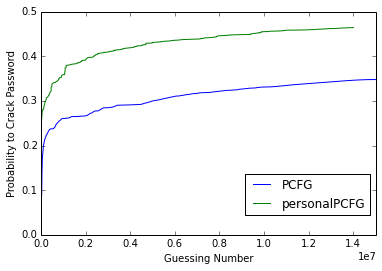
\includegraphics[width=.9\linewidth]{fig/cmp}

\end{minipage}
\begin{minipage}{.33\textwidth}
  \captionsetup{font=scriptsize}
  \centering
  \caption{PCFG and Personal-PCFG -- Online attacks.}{}
  \label{cmp100}
  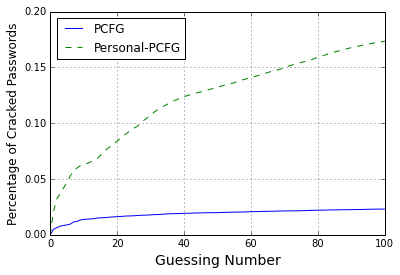
\includegraphics[width=.9\linewidth]{fig/cmp100}

\end{minipage}%
\begin{minipage}{.33\textwidth}
  \captionsetup{font=scriptsize}
  \centering
  \caption{Representative Points -- Online attacks.}{}
  \label{points}
  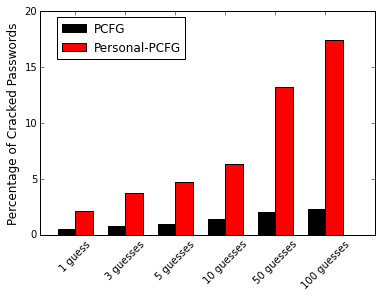
\includegraphics[width=.9\linewidth]{fig/online}
\end{minipage}
\end{figure*}



\begin{enumerate}[leftmargin=*]
\item Both PCFG and Personal-PCFG can crack passwords quickly when they just start. However, the line become flat when the guessing number is growing large. This is not surprising because both methods try high probability guesses first. 

\item Personal-PCFG works much better than PCFG. With 10 million hashes Personal-PCFG achieves the probability that is achieved with over 300 million guesses by original PCFG method. That is to say, Personal-PCFG can crack password much much faster than PCFG method. 

\item Personal-PCFG is able to cover larger password space than PCFG method. This is because personal information provides rich personalized strings which may not appear in the training set.

\end{enumerate}

After illustrating the benefit of Personal-PCFG in offline attacks, we also show the effectiveness of Personal-PCFG in online attacks. Online attacks allow much less guessing attempts because a real system usually restrain login attempts for a specific user. Therefore we limit the guesses to be at most 100 times. In fact, most systems will not allow login attempts to exceed 10 time.s. We present the results in Figure~\ref{cmp100}.


As shown in Figure~\ref{cmp100}, in online attacks, generally Personal-PCFG is able to crack 323\% to 649\% more passwords than original PCFG. We then take a look at several representative guessing numbers. These interesting points are shown in Figure~\ref{points}. A most typical system allows 5 attempts to input the correct passwords. Personal-PCFG is able to crack 4.7\% passwords within only 5 guesses. Meanwhile the percentage is only 0.9\% for original PCFG method. In addition, it would take over 800 guesses for PCFG to reach a success rate of 4.7\%. Clearly Personal-PCFG is more powerful to crack out the correct passwords within only a few guesses. 

To conclude, we show that Personal-PCFG beats PCFG in both online and offline attacks substantially. The only restriction of Personal-PCFG is that it requires personal information. However, we have showed personal information is not hard to obtain under our attack scenarios.


